\documentclass[10pt,twocolumn]{article}
\usepackage[margin=0.72in]{geometry}
\usepackage{amsmath}
\usepackage{amssymb}
\usepackage{booktabs}
\usepackage{tikz}
\usetikzlibrary{positioning}
\title{A Small Layout-Preservation Test}
\author{Codex Bilingual Reader Test Fixture}
\date{}
\begin{document}
\maketitle
\begin{abstract}
This paper tests a bilingual PDF workflow. It contains two columns, a display formula, a vector figure, and a table. The original mathematical notation must survive translation.
\end{abstract}
\section{Method}
Let $x \in \mathbb{R}^d$ be a visual feature. We preserve the equation
\begin{equation}
E = mc^2, \qquad p(y \mid x) = \frac{\exp(y^\top x)}{\sum_{k=1}^{K}\exp(k^\top x)}.
\label{eq:energy}
\end{equation}
The surrounding English prose should be translated into Simplified Chinese without modifying Equation~\ref{eq:energy}. Figure~\ref{fig:pipeline} is a vector drawing and should remain visible in the output PDF.

\begin{figure}[t]
\centering
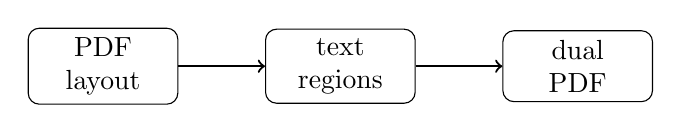
\begin{tikzpicture}[node distance=11mm, every node/.style={draw, rounded corners, align=center, minimum width=19mm, minimum height=7mm}]
\node (pdf) {PDF\\layout};
\node[right=of pdf] (text) {text\\regions};
\node[right=of text] (out) {dual\\PDF};
\draw[->, thick] (pdf) -- (text);
\draw[->, thick] (text) -- (out);
\end{tikzpicture}
\caption{A vector pipeline figure with labels.}
\label{fig:pipeline}
\end{figure}

\section{Results}
Table~\ref{tab:result} has text that is safe to translate. The numbers and the formula symbols should remain intact.
\begin{table}[h]
\centering
\begin{tabular}{lrr}
\toprule
Method & Accuracy & $F_1$ \\
\midrule
Baseline & 71.2 & 68.4 \\
Proposed method & 78.6 & 75.9 \\
\bottomrule
\end{tabular}
\caption{Quantitative results for the test document.}
\label{tab:result}
\end{table}

The page must keep its column structure, formulas, table borders, captions, and the original vector drawing. This final paragraph provides ordinary text for translation and wraps across lines.
\end{document}
